\documentclass{beamer}
\usepackage[T1]{fontenc}
\usepackage[english]{babel}
\usefonttheme{serif}
\setbeamertemplate{navigation symbols}{
\usebeamerfont{footline}
\usebeamercolor[fg]{footline}
\insertframenumber/\inserttotalframenumber{}
}
\setbeamerfont{frametitle}{size = \small}
\usepackage{mathpazo}
\usepackage{float}
\usepackage[labelsep = colon]{caption}
\usepackage{amsmath}
\usepackage{setspace}
\usepackage{graphicx}
\usepackage{threeparttablex}
\usepackage{longtable}
\usepackage{booktabs}
\usepackage{dcolumn}
\usepackage{pdfpages}


\title{GV217 Conflict Analysis}
\subtitle{Week 17: The Decline of Conflict}
\author{Muzhou Zhang\\ muzhou.zhang@essex.ac.uk\\ Virtual Office Hour: 15:30--16:30, Friday, 997 5800 8679}
\date{28 Jan 2022}

\begin{document}
\maketitle
\setstretch{1.25}

\begin{frame}{Declining Conflict: Description}
    \pause
    \begin{center}
        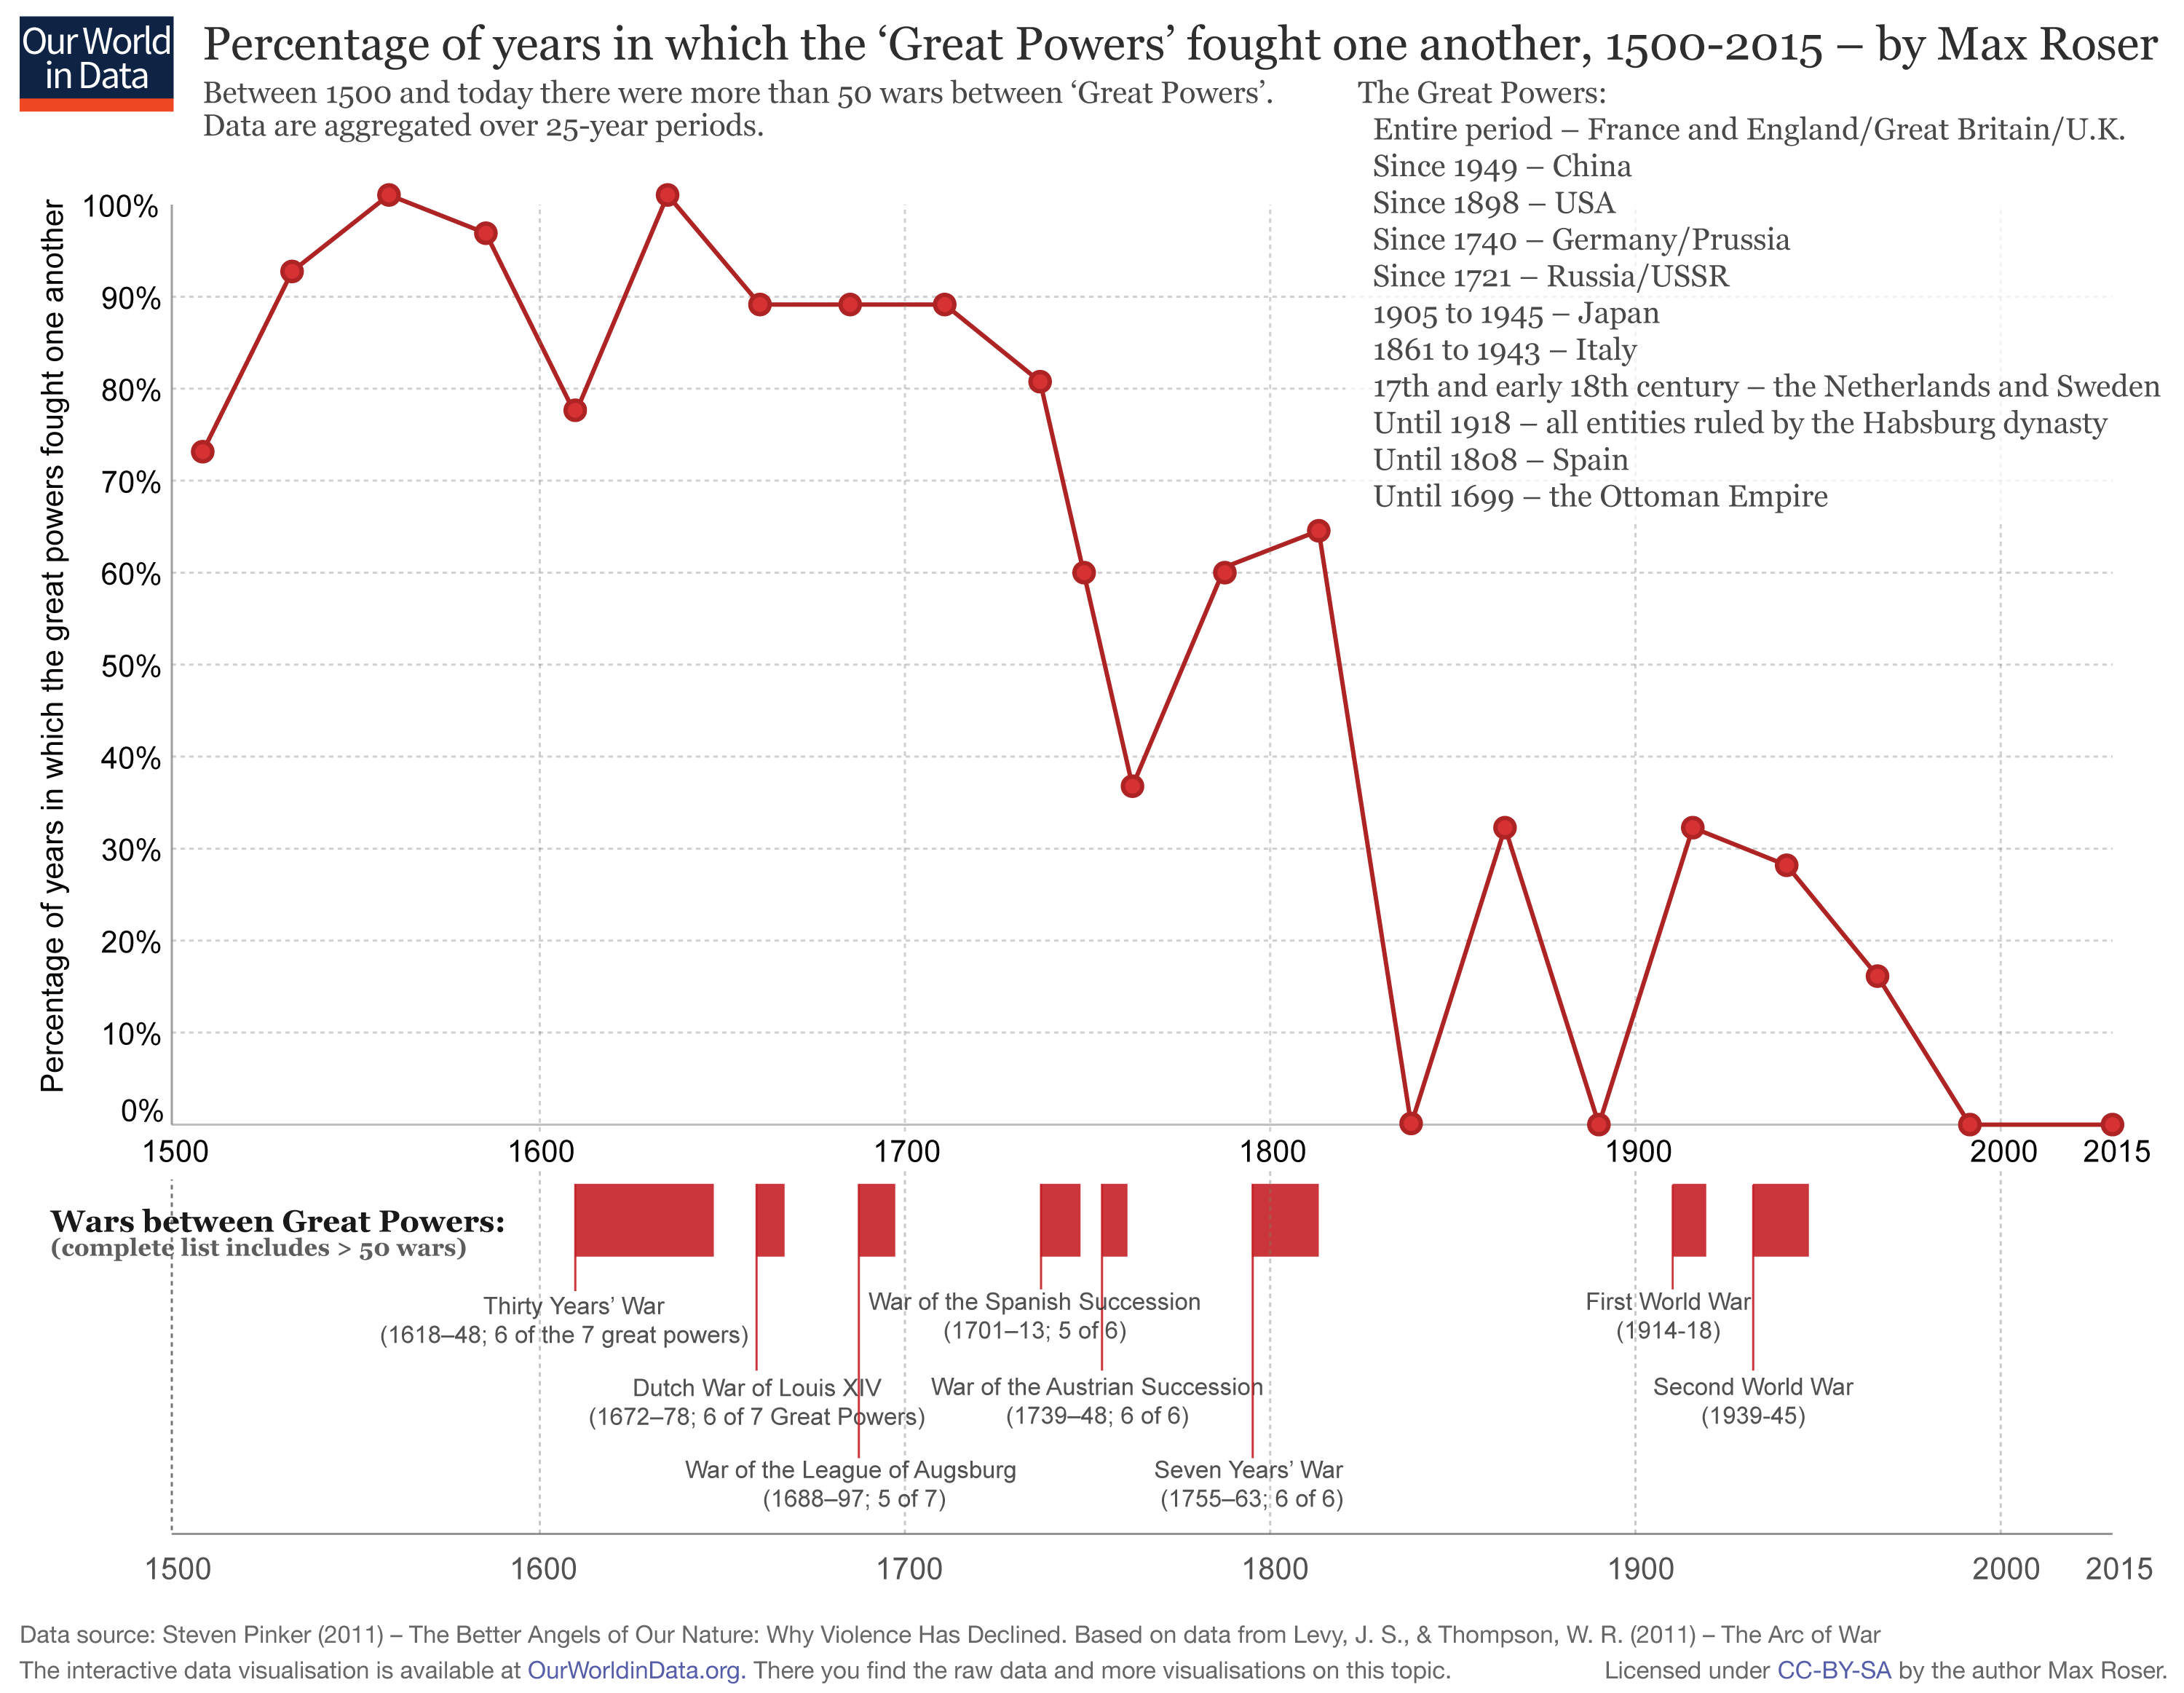
\includegraphics[width = \linewidth]{/Users/mz/Desktop/GitHub/teaching/gv217_conflict_analysis/figs/fig1_wk17.png}
    \end{center}
\end{frame}

\begin{frame}{Declining Conflict: Description}
    \pause
    \begin{center}
        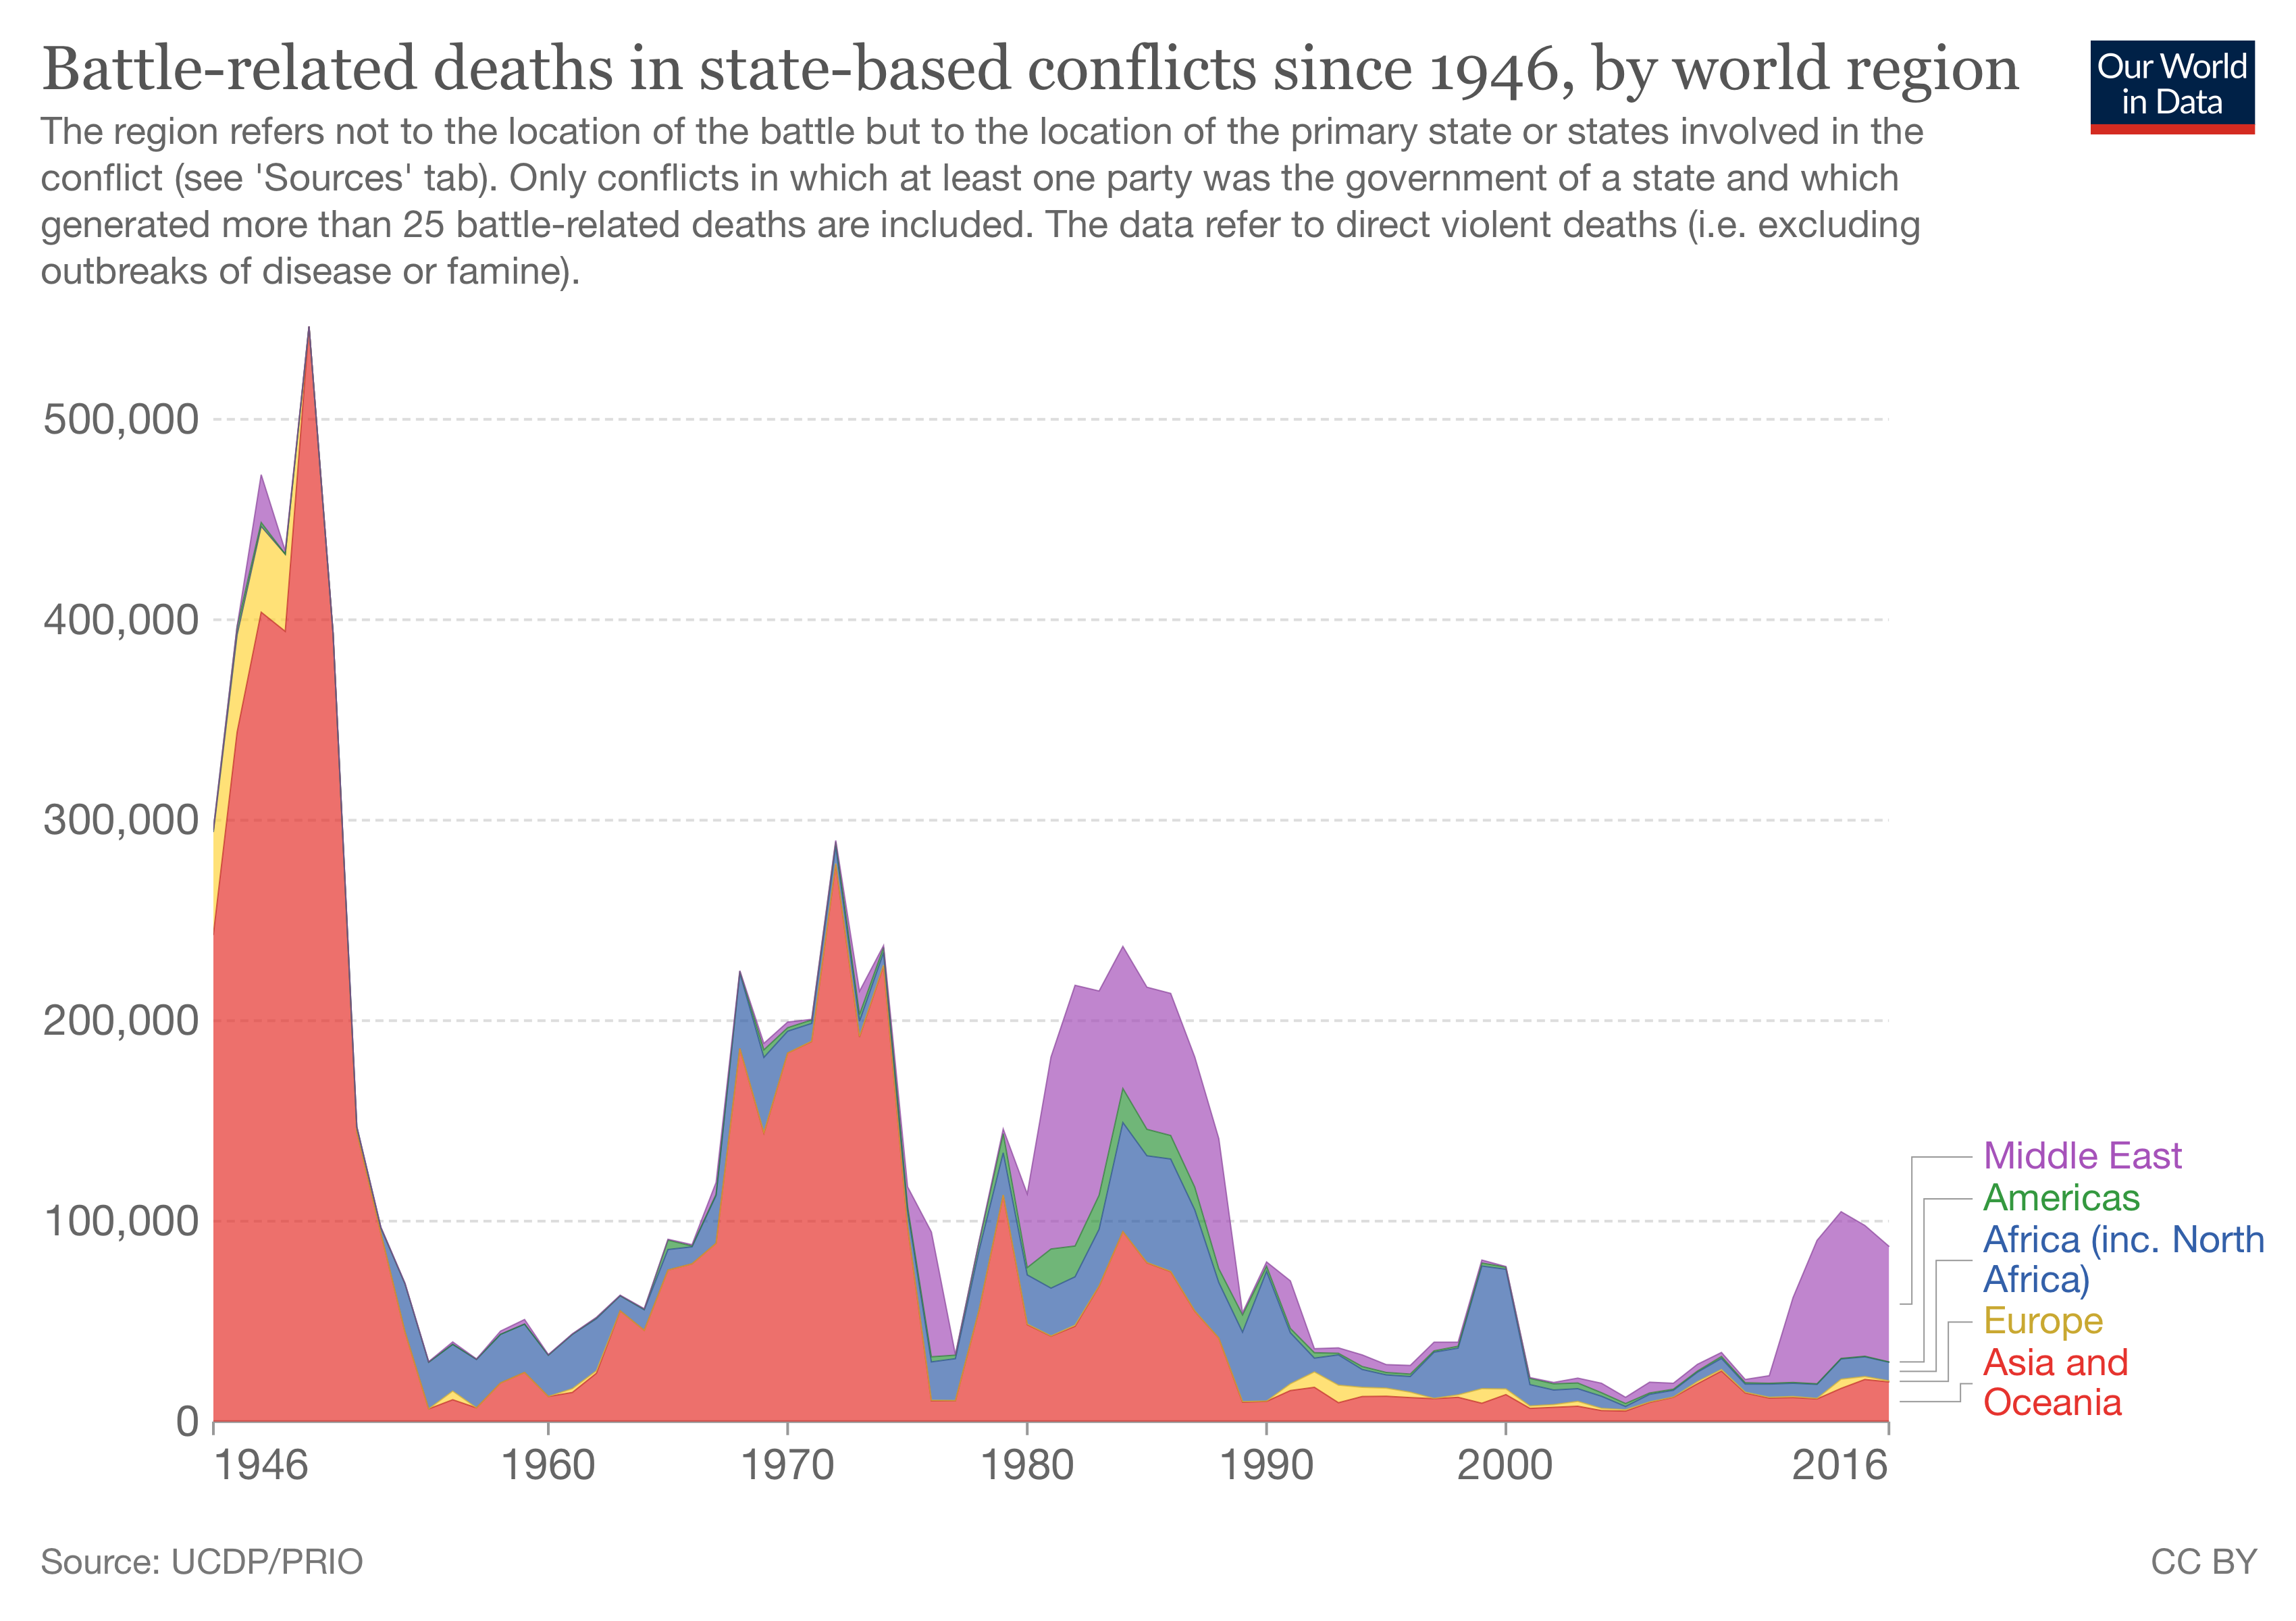
\includegraphics[width = \linewidth]{/Users/mz/Desktop/GitHub/teaching/gv217_conflict_analysis/figs/fig2_wk17.png}
    \end{center}
\end{frame}

\begin{frame}{Declining Conflict: Causation}
    \begin{itemize}
        \pause\item The modern state
        \pause\item Democratic peace
        \pause\item Capitalist peace
        \pause\item Women's empowerment
        \pause\item Education and norm diffusion
    \end{itemize}
\end{frame}

\begin{frame}{Is Conflict Declining?}
    \pause
    \begin{center}
        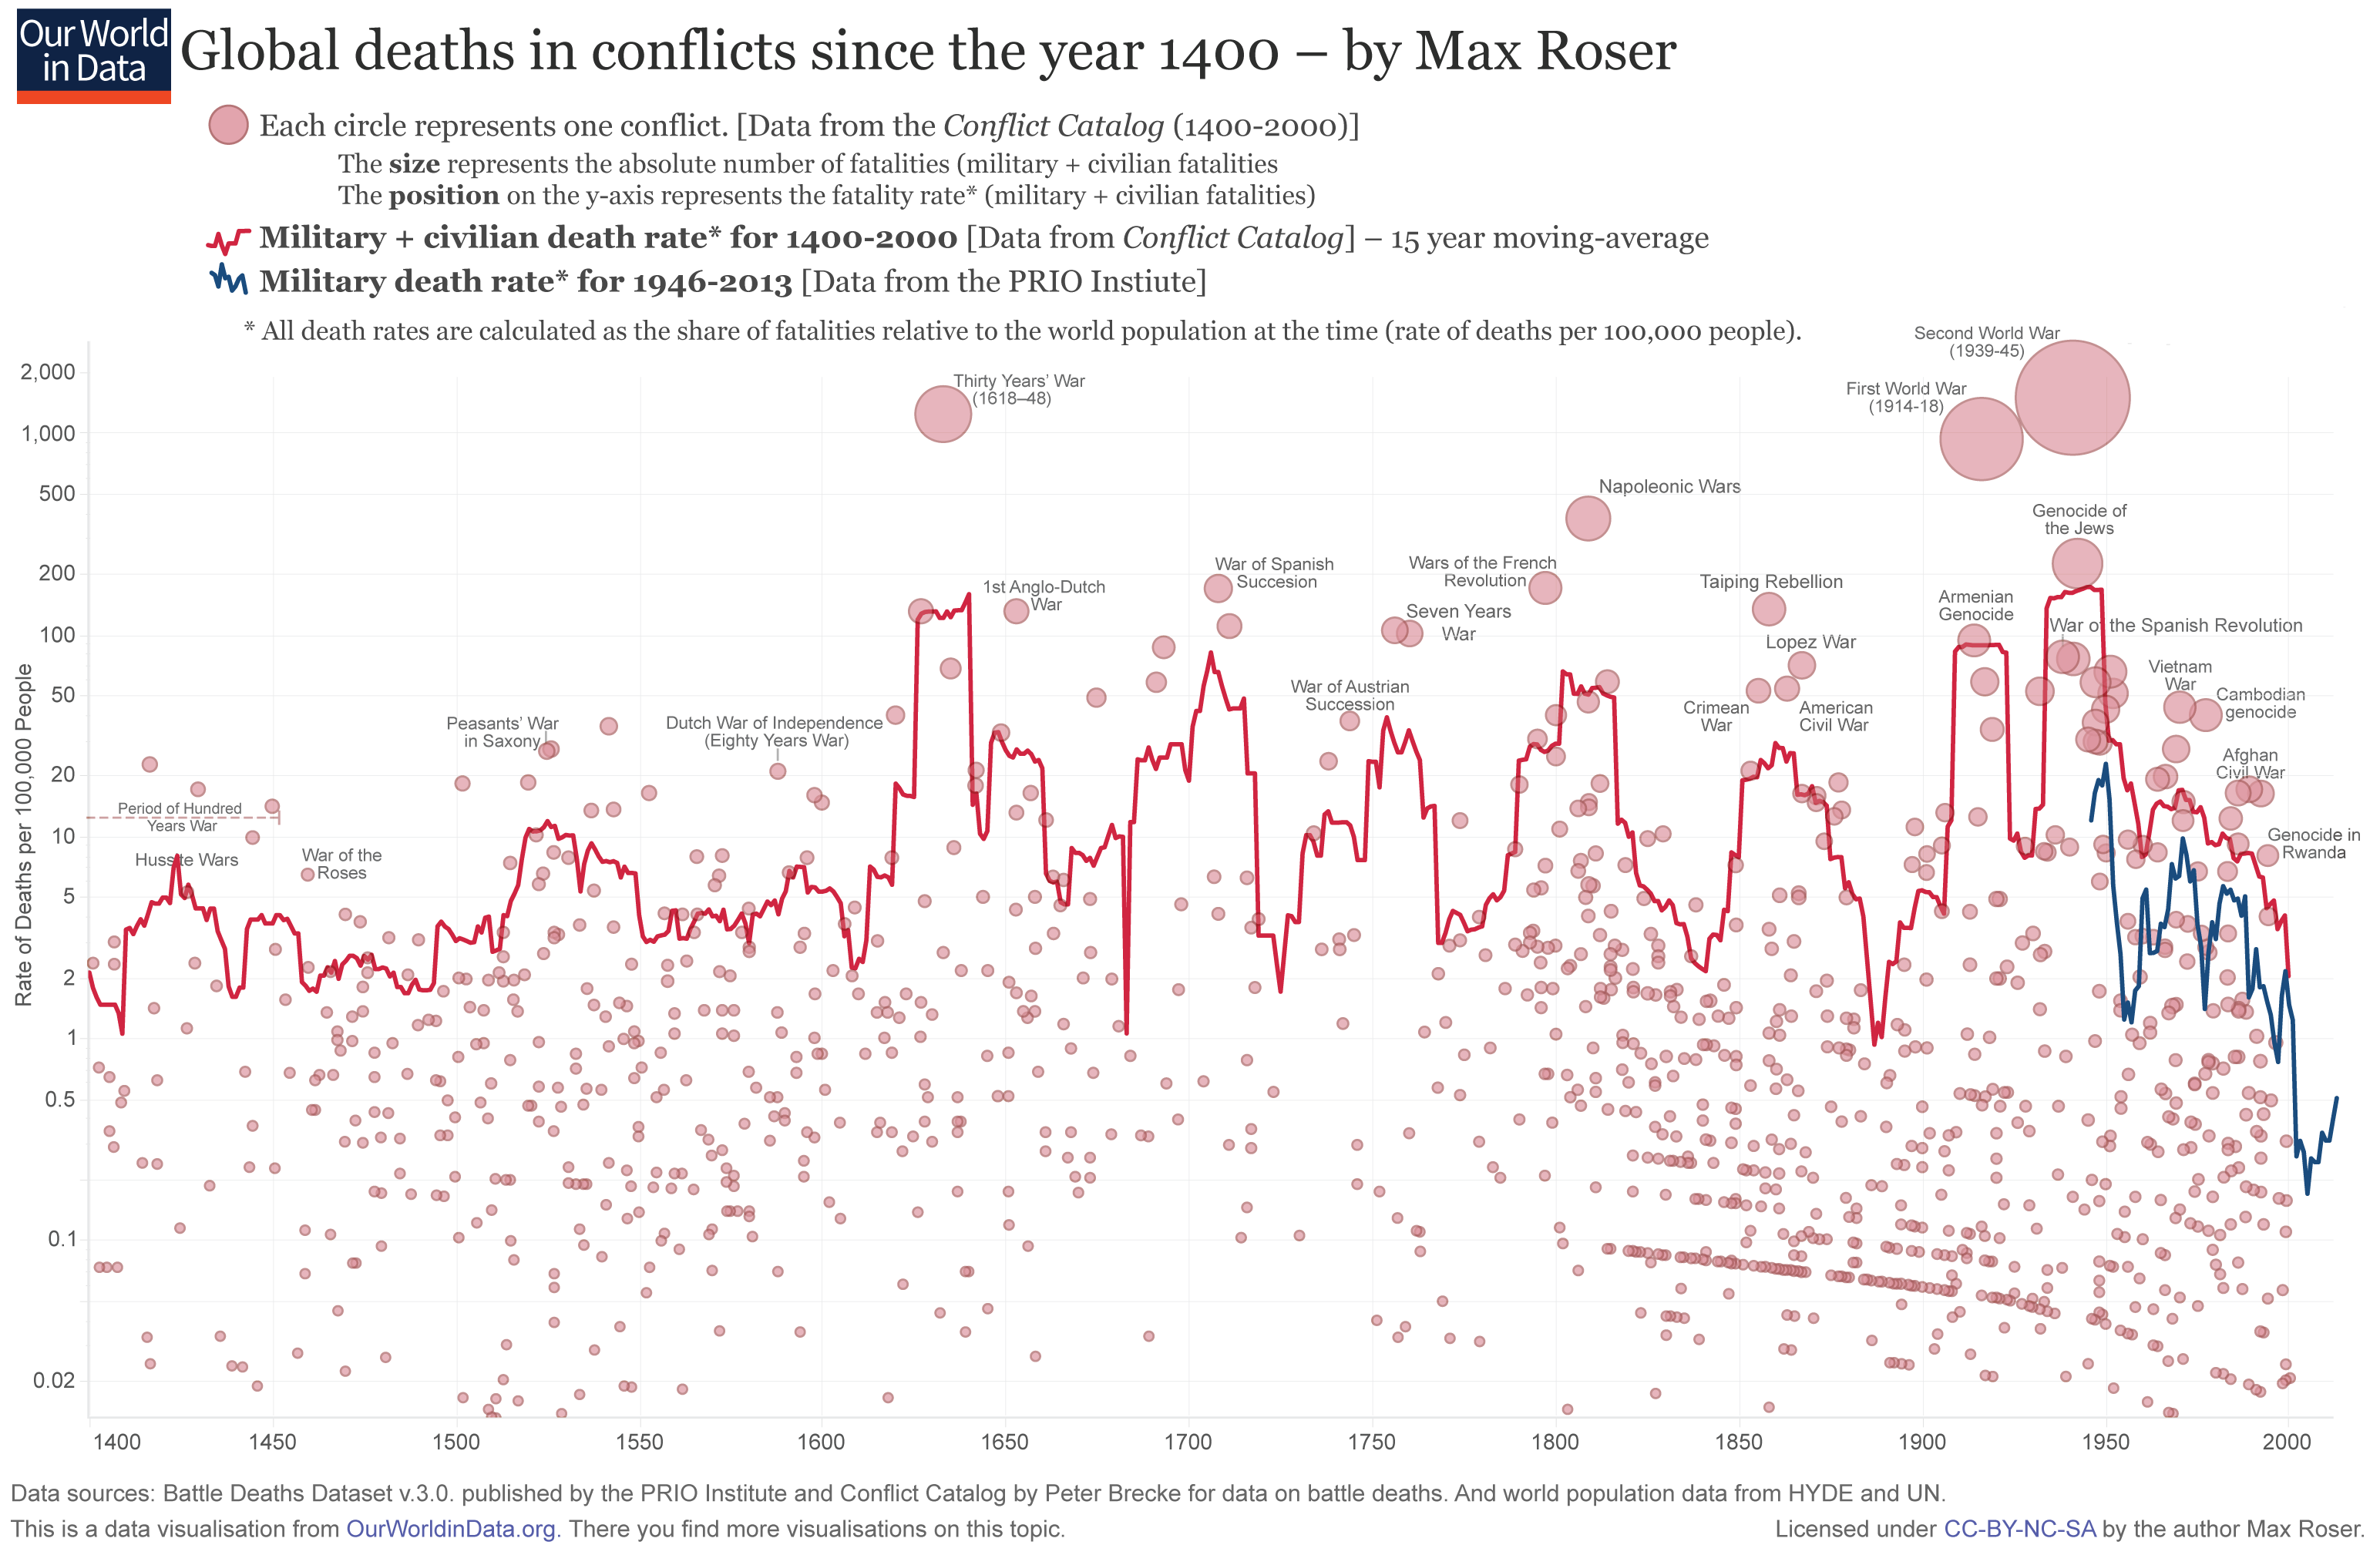
\includegraphics[width = \linewidth]{/Users/mz/Desktop/GitHub/teaching/gv217_conflict_analysis/figs/fig3_wk17.png}
    \end{center}
\end{frame}

\begin{frame}{Is Conflict Declining?}
    \begin{itemize}
        \pause\item Different measures, inconsistent answers
        \pause\item Unreliable extrapolation
    \end{itemize}
\end{frame}

\begin{frame}{UCDP Data: What}
    \pause\url{https://ucdp.uu.se/downloads}
    \pause
    \begin{center}
        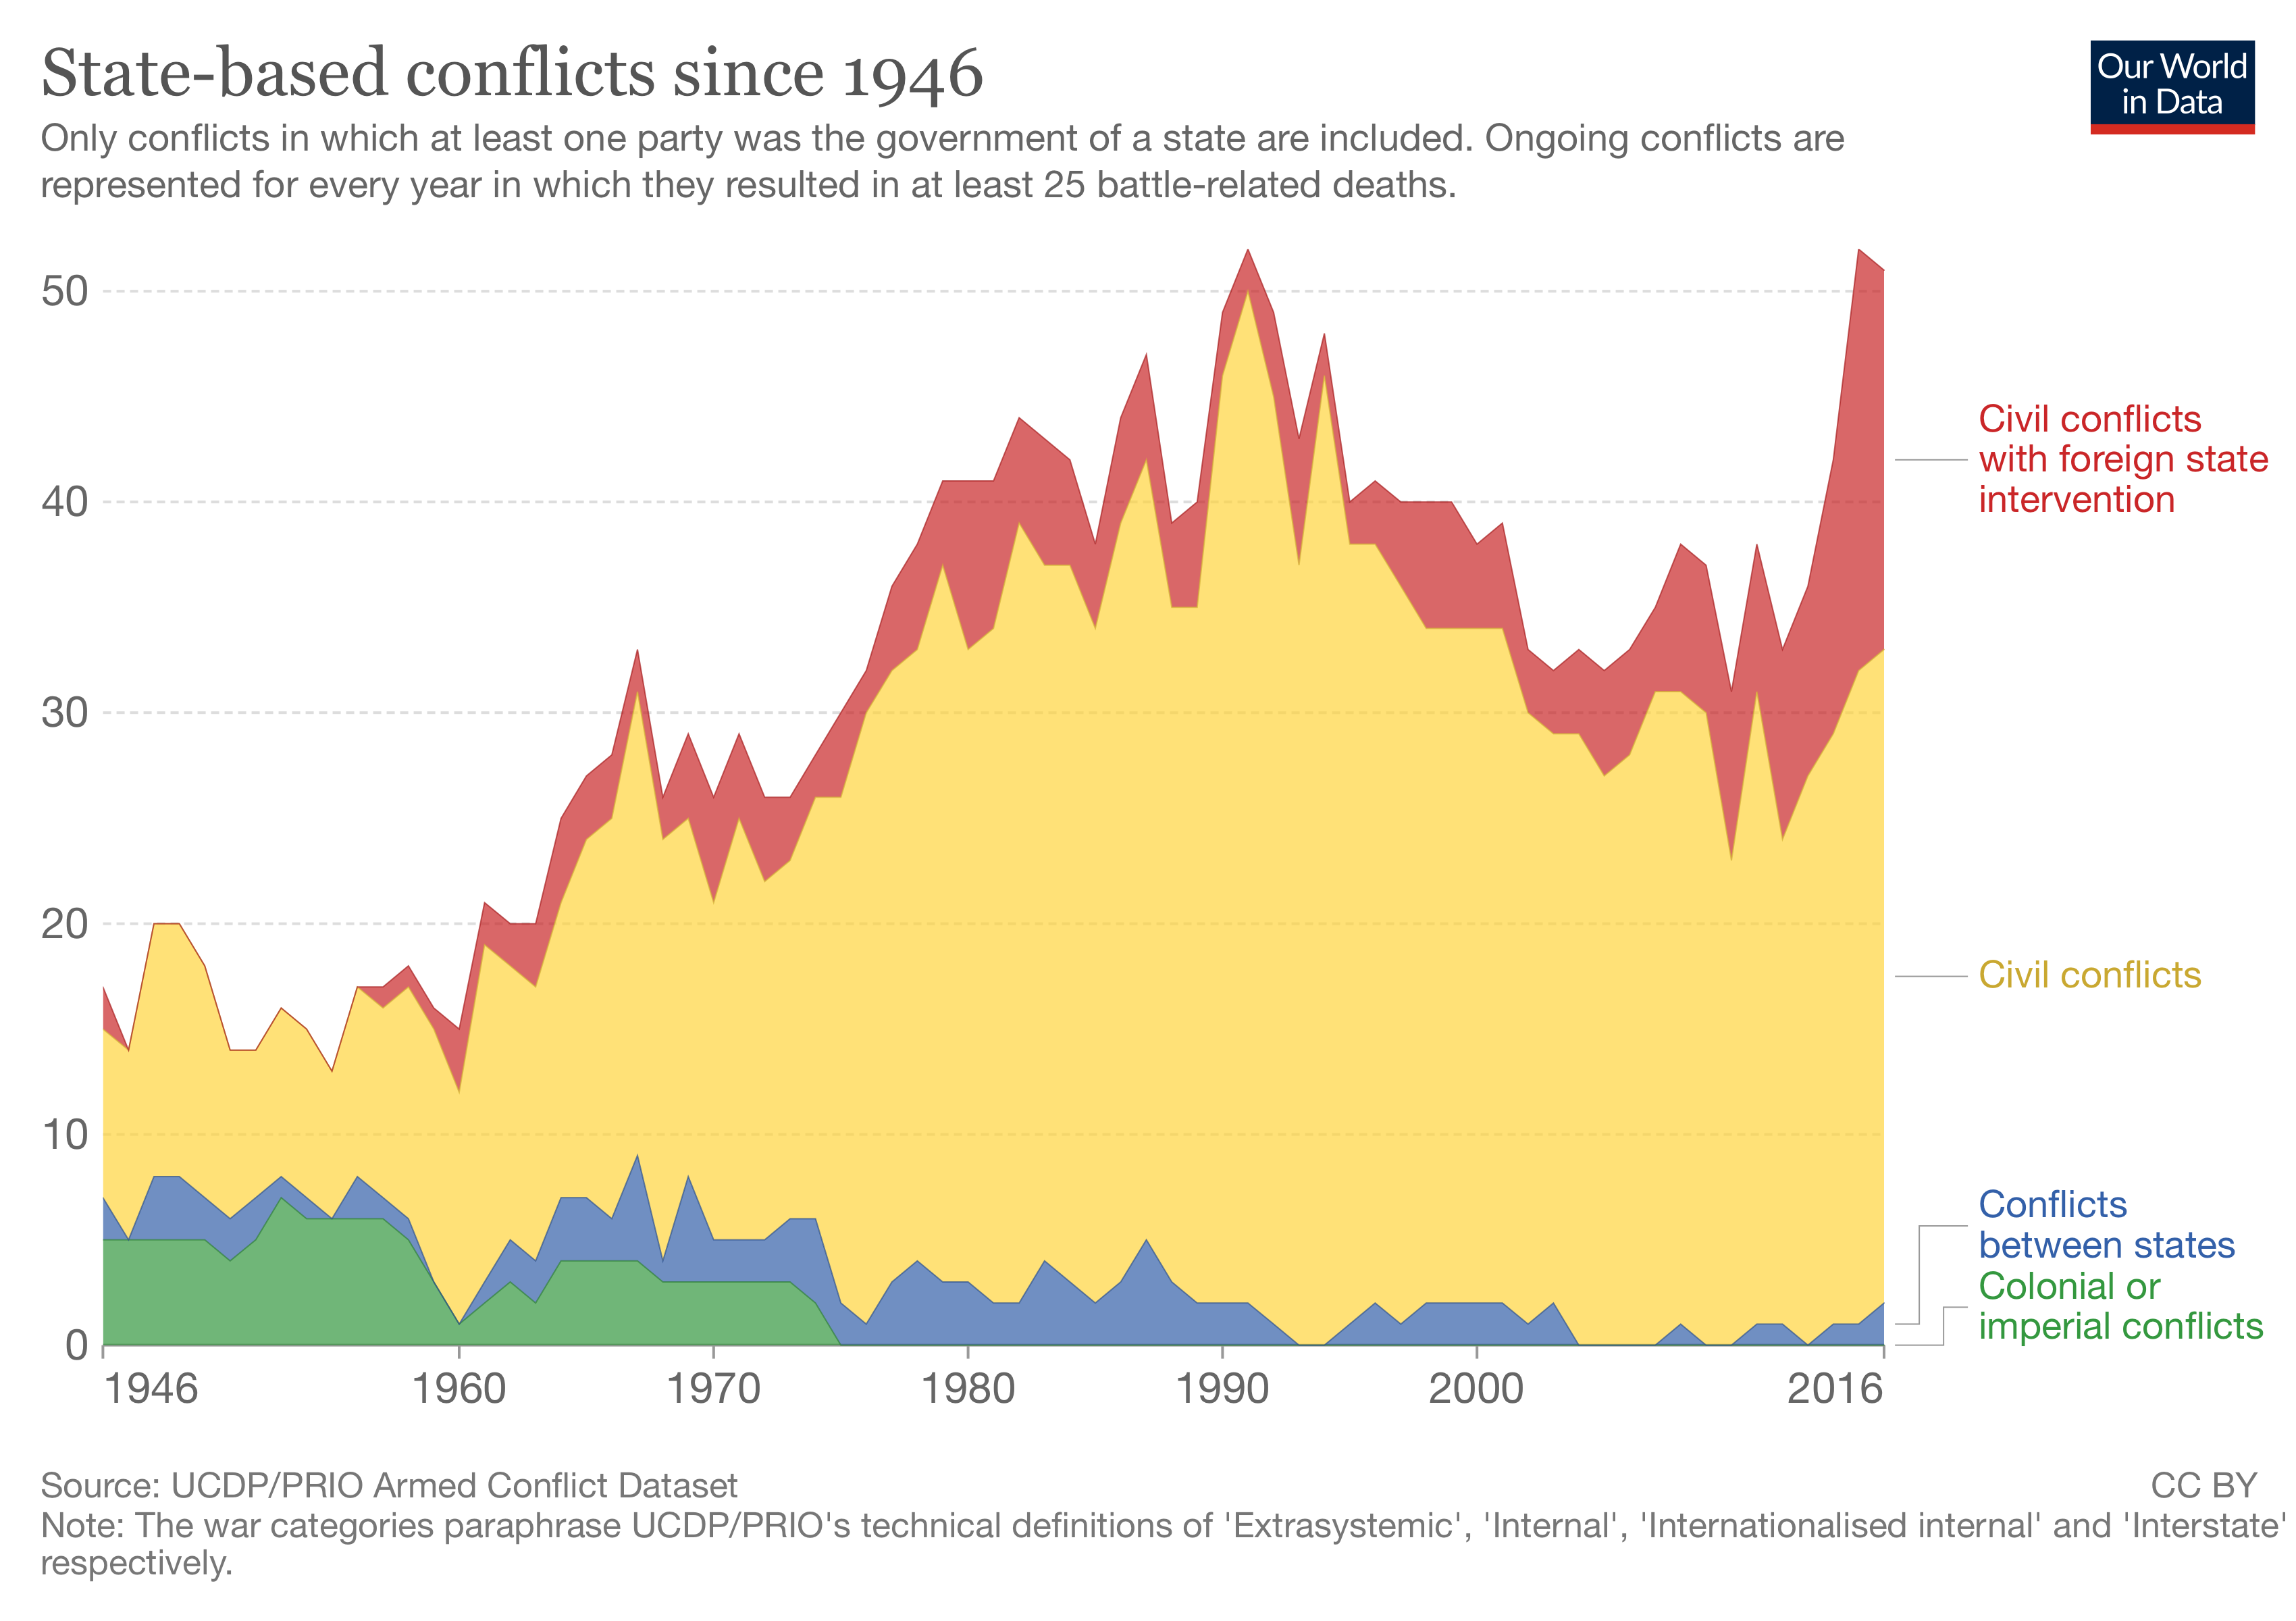
\includegraphics[height = 0.65\linewidth, width = \linewidth]{/Users/mz/Desktop/GitHub/teaching/gv217_conflict_analysis/figs/fig4_wk17.png}
    \end{center}
\end{frame}

\begin{frame}{UCDP Data: Classification}
    \pause
    \begin{center}
        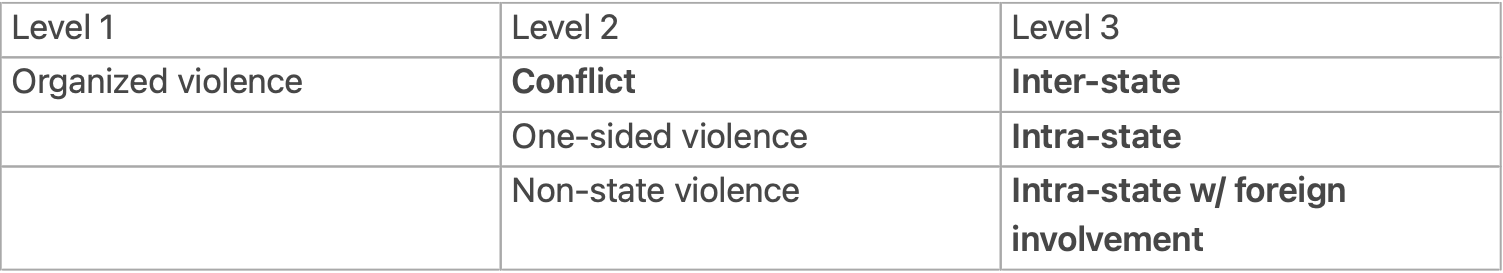
\includegraphics[width = \linewidth]{/Users/mz/Desktop/GitHub/teaching/gv217_conflict_analysis/figs/fig5_wk17.png}
    \end{center}
\end{frame}

\begin{frame}{UCDP Data: What Is Conflict}
    \begin{itemize}
        \pause\item Incompatibility concerning government or territory
        \pause\item State-based at least on one side
        \pause\item At least 25 battle death
        \pause\item Violent on both sides
    \end{itemize}
\end{frame}

\begin{frame}{UCDP Data: Are They Conflict?}
    \begin{itemize}
        \pause\item Poisoning of Sergei and Yulia Skripal, Salisbury, 2018
        \pause\item The war on drugs, Mexico
        \pause\item China-India border stand-off, 2010s--2020s
        \pause\item Battle of Aleppo (2012-–2016)
    \end{itemize}
\end{frame}

\begin{frame}{UCDP Data: Event-level}
    \pause
    \begin{center}
        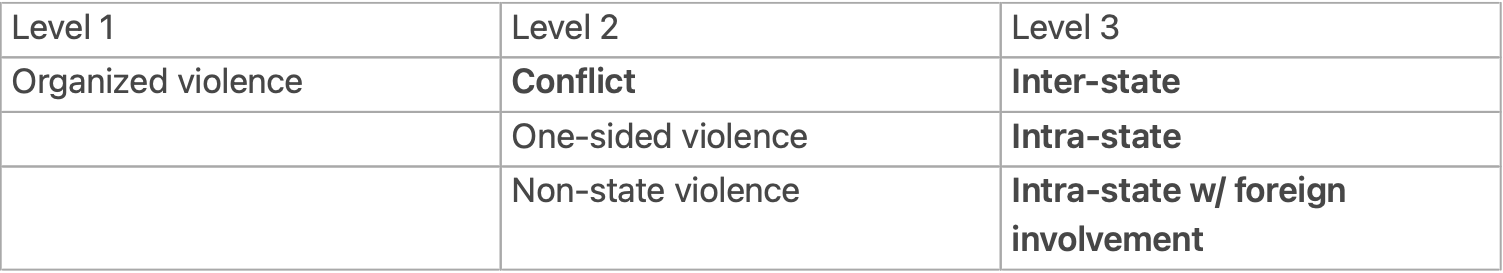
\includegraphics[width = \linewidth]{/Users/mz/Desktop/GitHub/teaching/gv217_conflict_analysis/figs/fig6_wk17.png}
    \end{center}
\end{frame}

\begin{frame}{Final Assessment}
    \begin{itemize}
        \pause\item Theory-driven case study
        \pause\item Analytical, not descriptive
        \pause\item Conflict as unit of analysis
    \end{itemize}
\end{frame}

\end{document}
